\section{实验数据与图像处理工作流}

\subsection{工作流概览}

图~\ref{fig:surrogate-data-flow} 展示了本文所用代理模型工作流的整体数据流，整个流程按四条泳道组织。
原始输入（高速 Mie 视频、标定配置和试验元数据）先经过 CUDA 加速的图像处理，生成一维特征和边界点；在此基础上，再得到基于二值化（BW）和基于 CDF 的穿深轨迹以及其他几何度量。
这些观测量通过无参数曲线拟合扩展为合成轨迹，并用于驱动三阶段神经网络训练：阶段~1（MSE）、阶段~2（NLL）和阶段~3（Raw + KD，知识蒸馏）。
最终训练得到的模型被部署到壁面碰撞筛查应用中，结合活塞几何和物理参数输出碰撞概率与可视化动画。
表~\ref{tab:workflow} 以文字形式总结了同样的阶段。
本章聚焦图~\ref{fig:surrogate-data-flow} 的前两条泳道：OSCC 视频数据如何完成标定、预处理、配准并转换为逐羽流分辨的几何观测量。
轨迹目标构造、代理建模训练和概率筛查则留到下一章展开。

方法层面的动机在于，光学实验能够提供基于图像的证据，但逐事件的图像后处理最终只会得到一个离散观测表。
如果停留在这一层，这些观测值不能直接作为条件参数化的预测模型用于快速设计迭代。
因此，本章把图像处理视为一层可审计的方法环节，而不是附属的预处理步骤；它负责将高速 Mie 记录转换为定义一致的逐羽流时序观测量。

这些任务基于 Wärtsilä 光学喷雾燃烧舱（OSCC）的数据完成。
原始材料是 TB 级、室温、非反应、顶视 Mie 散射记录，在固定相机布置下跨多个工况和喷嘴几何采集得到。
整条链路先手动标定喷嘴几何，再通过 CUDA 加速预处理、极坐标配准和羽流条带提取生成逐羽流观测量，
并通过降阶拟合构造穿深目标，随后交给第~4 章所述的三阶段 MLP surrogate。

\begin{figure}[t]
\centering
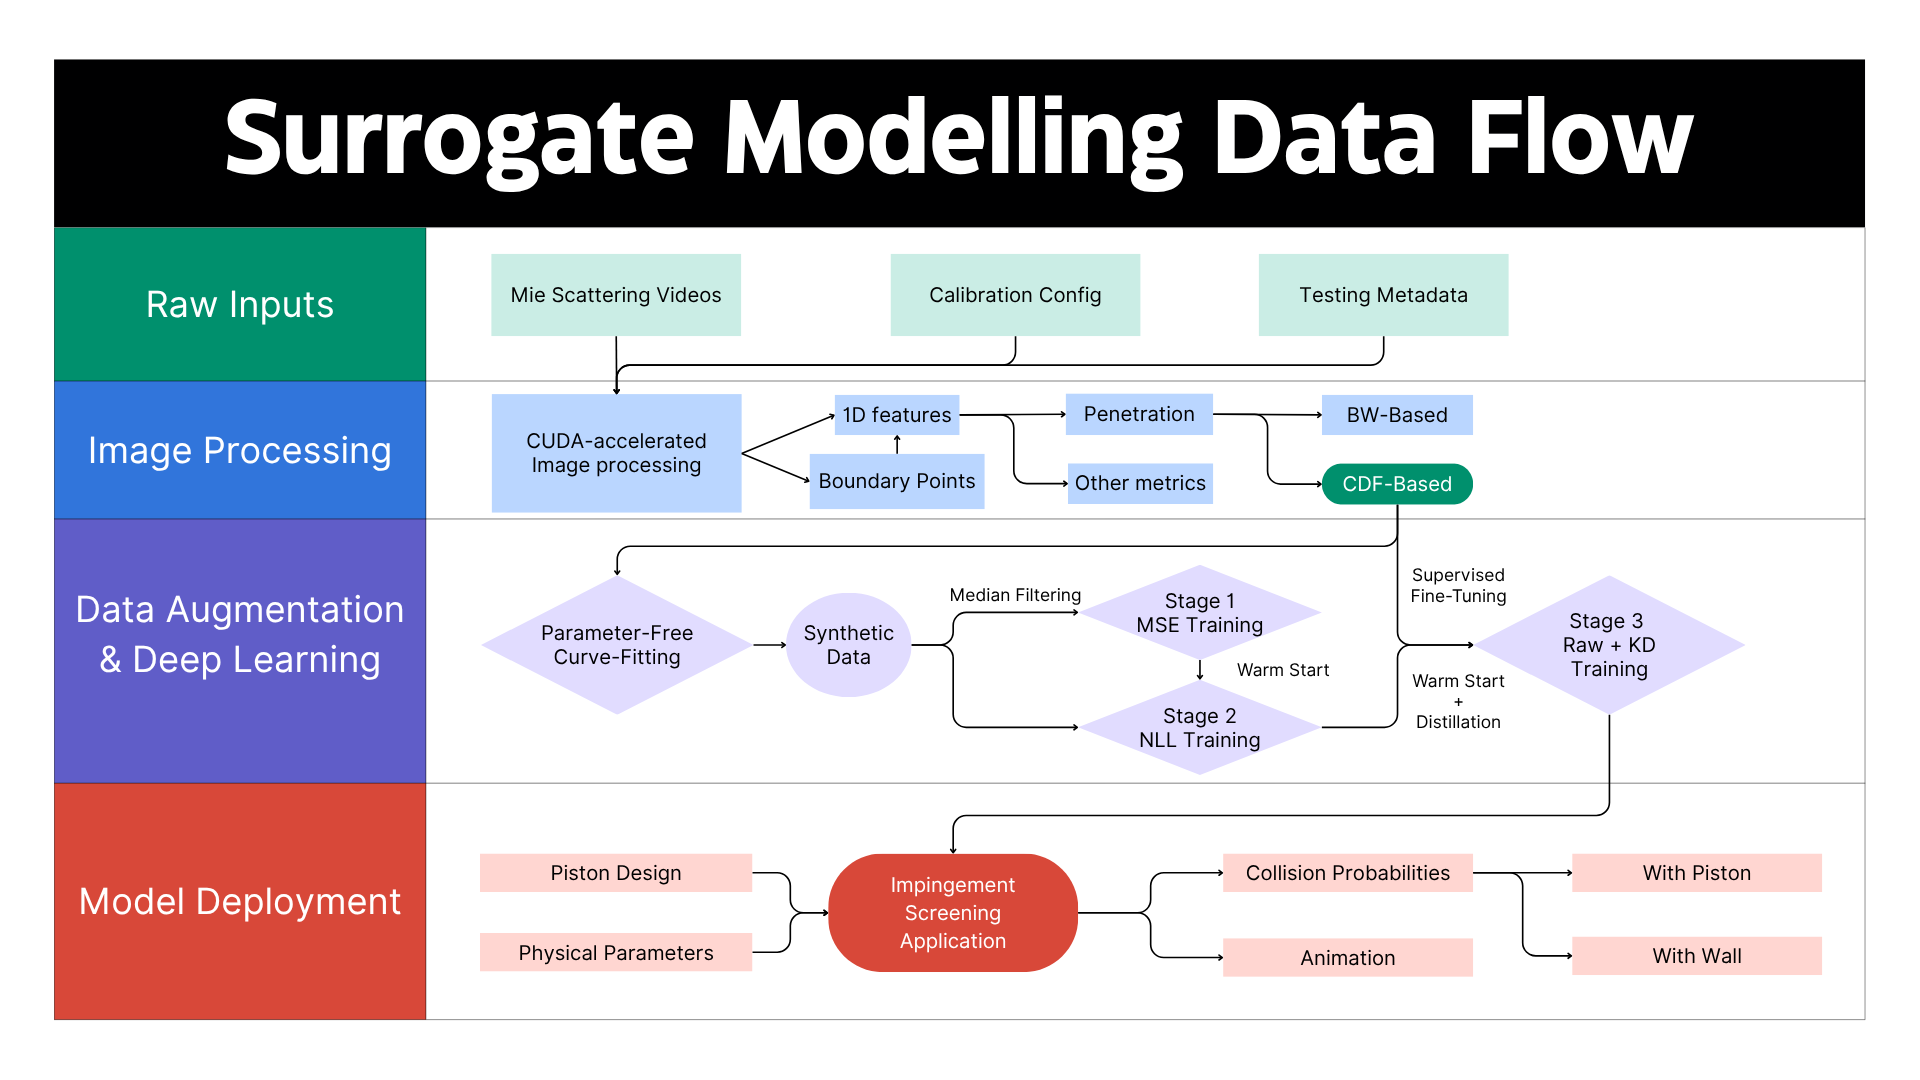
\includegraphics[width=\linewidth]{../images/surrogate_modelling_data_flow.png}
\caption{代理模型数据流总览。四条泳道分别对应原始输入、图像处理、数据增强与深度学习，以及模型部署；箭头标注了关键的数据传递和训练连接关系（Median Filtering、Warm Start、Warm Start + Distillation、Supervised Fine-Tuning）。}
\label{fig:surrogate-data-flow}
\end{figure}

\begin{table}[t]
\centering
\begin{tabular}{|L{0.21\linewidth}|L{0.26\linewidth}|L{0.33\linewidth}|}
\hline
阶段 & 主要作用 & 主要输出 \\
\hline
手动喷嘴标定 & 固定喷嘴中心、半径和角向参考 & 每个记录集对应一个几何锚点 \\
\hline
批量视频处理与羽流提取 & 批量预处理、逐羽流特征提取和边界导出 & 按羽流分解的穿深轨迹、二值几何指标和边界 CSV \\
\hline
轨迹清洗与降阶拟合 & 清洗、时延对齐和删失感知目标构造 & 清洗后的轨迹、拟合参数和拟合图 \\
\hline
阶段~1 MSE 基线 & 确定性的代表轨迹训练 & 训练日志、scaler 状态、\codepath{best\_model\_stage1.pt} 和 loss 曲线 \\
\hline
阶段~2 NLL 扩展 & 在完整过滤数据集上学习异方差均值和方差 & 训练日志、scaler 状态和教师 checkpoint \codepath{best\_model\_stage2.pt} \\
\hline
阶段~3 蒸馏精化 & 区间依赖的原始 CDF 蒸馏和早期时间细化 & 运行日志、\codepath{best\_model\_refinement.pt} 和消融摘要 \\
\hline
原型概率筛查 & 将预测的穿深分布投影到简化发动机几何上以评估近壁风险 & 逐帧 $P_{\mathrm{hit}}(t)$、累计 $E$ 和可视化动画 \\
\hline
\end{tabular}
\caption{本文记录的已实现工作流。}
\label{tab:workflow}
\end{table}

\subsection{实验数据集}

输入数据来自 Wärtsilä 测试设施运行的加压喷雾燃烧舱（OSCC）。
共测试了九个喷嘴族：八个原型喷嘴（Nozzle1--Nozzle8），记录于 2024 年 10--11 月，
以及一个参考喷油器（Nozzle0），记录于 2022 年 6 月。
表~\ref{tab:nozzle-overview} 总结了每个喷嘴族的几何形状及覆盖的工况范围。

\begin{table}[t]
\centering
\footnotesize
\setlength{\tabcolsep}{4pt}
\renewcommand{\arraystretch}{1.1}
\begin{tabular}{@{}lcccccc@{}}
\toprule
喷嘴 & $d_n$ (mm) & $N$ & $\theta_{\mathrm{umb}}$ (°) & FPS & $P_{\mathrm{inj}}$ (bar) & $t_{\mathrm{inj}}$ (\si{\micro s}) \\
\midrule
Nozzle1 & 0.384 & 10 & 140 & 25{,}000 & 2000          & 560--779   \\
Nozzle2 & 0.375 & 10 & 140 & 25{,}000 & 1400--2000    & 500--917   \\
Nozzle3 & 0.365 & 10 & 140 & 25{,}000 & 2000          & 580--764   \\
Nozzle4 & 0.355 & 10 & 140 & 25{,}000 & 2000          & 558--745   \\
Nozzle5 & 0.348 & 11 & 140 & 25{,}000 & 2000          & 570--763   \\
Nozzle6 & 0.333 & 12 & 140 & 25{,}000 & 2000          & 609--881   \\
Nozzle7 & 0.365 & 12 & 164 & 25{,}000 & 2000          & 580--764   \\
Nozzle8 & 0.365 & 10 & 130 & 25{,}000 & 2000          & 580--764   \\
Nozzle0 & 0.384 & 10 & 140 & 34{,}000 & 1400--2200    & 340--1200  \\
\bottomrule
\end{tabular}
\caption{喷嘴几何与工况范围。$d_n$：孔径；$N$：喷孔数；$\theta_{\mathrm{umb}}$：伞角（umbrella angle）；FPS：记录帧率；$P_{\mathrm{inj}}$：喷射压力；$t_{\mathrm{inj}}$：指令喷射时长。腔压范围为 4.42--13.26\,bar（Nozzle1--8，三个密度层级）和 5--35\,bar（Nozzle0）。Nozzle0 的控制背压为 1\,bar 或 4\,bar；Nozzle1--8 未独立改变控制背压。}
\label{tab:nozzle-overview}
\end{table}

在这九个喷嘴族中，喷射压力范围为 1,400 到 2,200\,bar，
指令喷射时长为 340 到 1,200\,\si{\micro s}，
腔压范围为 4.42 到 35\,bar。
每个工况子文件夹通常包含五次重复记录，
每段记录都会裁剪到约 100 帧，以限制 GPU 内存占用。
处理后的归档总计包含 266 个试验工况子文件夹和 2,992 个记录文件
（每个 \texttt{.cine} 对应一个 CSV）；裁剪后的工作归档占据数十 GB，
而完整未裁剪记录则是 TB 级原始输入。
最新统计会在每次运行 \textbf{数据清洗与拟合程序} 结束时，由 \textbf{数据集汇总脚本} 自动重新生成。

\subsection{喷嘴几何的人工标定}\label{subsec:nozzle-calibration}

\textbf{交互式标定界面}中的手动标定工作流包含三个面向用户的阶段。

首先，操作者在主标注界面中打开代表性帧，调整显示设置，并准备好用于批量锚定的喷嘴中心视图。

其次，启动专用标定对话框，用户在选定帧上点击喷嘴边缘点。

第三，拟合得到的中心和半径回传到主界面，操作者在保存配置前，可将恢复出的几何与羽流导向线、环形叠加一起检查。

点选择对话框至少要求三次点击；在输入所需点数后，程序通过 \textbf{代数圆拟合函数} 计算圆。
拟合后的圆提供整个记录的喷嘴中心、标定半径和角度偏移。

\begin{figure}[t]
\centering
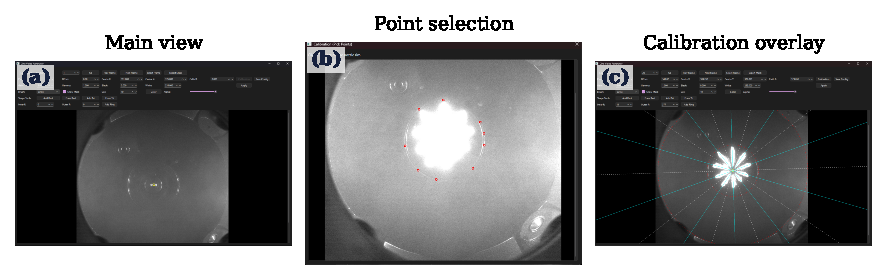
\includegraphics[width=\linewidth]{../images/fig_gui_calibration_workflow.pdf}
\caption{交互式喷嘴标定工作流。（a）主界面载入代表性帧并调整显示；（b）点选择对话框记录喷嘴边缘点；（c）圆拟合结果、羽流导向线和环形叠加被写回主界面，用于检查后续批量处理所用的几何锚点。}
\label{fig:gui-calibration-workflow}
\end{figure}

这种设计适合当前数据集，因为一次记录内相机和喷油器几何保持固定，而且背景里有若干与喷嘴同心的工件可以作为辅助参考。
只标定一次、并为所有帧复用同一个中心，可以避免下游羽流角度分析中的帧间抖动。

\subsection{批量视频处理与羽流提取}

\begin{figure}[t]
\centering
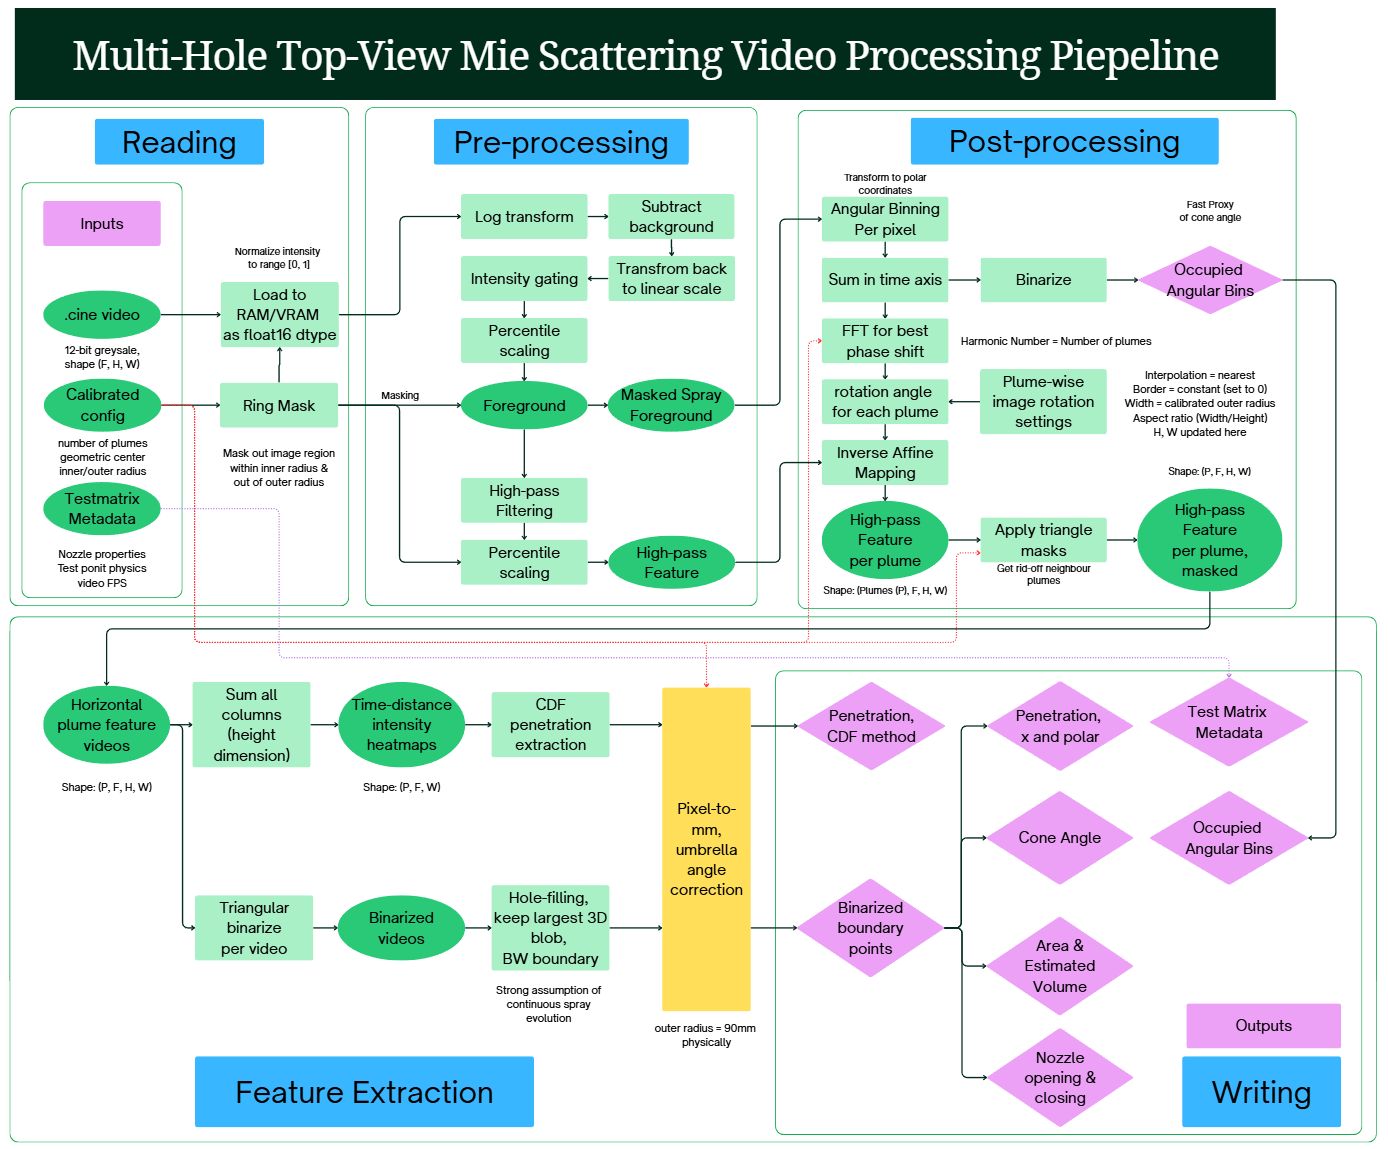
\includegraphics[width=1\linewidth]{../images/Multi-Hole Top-View Mie Scattering Video Processing Pipeline.png}
\caption{多孔顶视 Mie 散射处理流程总览，从原始 \texttt{.cine} 录像，经标定、CUDA 加速预处理、羽流配准和穿深提取，直到 CSV 导出。}
\label{fig:pipeline-overview}
\end{figure}

\textbf{多孔几何构建脚本}中的文件处理器是图像分析工作流的运行中枢。
对于每个 \texttt{.cine} 记录，\textbf{视频处理循环}会把视频加载到当前数组后端，复用整个文件夹的环形掩码，调用 \textbf{多孔预处理程序} 和 \textbf{多孔后处理程序}，提取逐羽流穿深曲线，计算基于边界的几何度量，并最终导出同步 CSV 和元数据文件。
这条链中数值开销最大的部分都尽量保留在后端本地：当 CuPy 可用时，卷积、角度分箱、重映射、阈值处理、连通域清理和形态学操作都会沿着 CUDA 路径执行，直到最终表格导出为止。

这一实现选择源自早期内部流程的实际限制。旧流程依赖逐帧 MATLAB 处理，缺少有效批量并行：处理约 50~GB 视频通常要花一天左右，而且容易崩溃。
因此，把重型图像操作迁移到批量 CUDA 导向流程中，在本文里属于方法设计，而不是单纯的软件优化。

\subsubsection{单块 GPU 上处理全量档案的四通道流水线方案}\label{subsec:concurrency-architecture}

流水线并行运行四个通道：磁盘预取、GPU 计算、CPU 特征提取和文件输出（图~\ref{fig:ch3-pipeline-lanes}）。GPU 处理当前录像时，磁盘工作线程同步加载下一段。GPU 处理完成后，输出文件在后台异步写入。若处理中途中断，检查点文件记录当前进度，支持从断点处续跑。

内存管理也与归档访问模式相匹配。
每处理完一条记录，临时数组会被释放，随后通过一次垃圾回收把 CuPy 数组归还到默认内存池；但块级池释放会故意推迟到子文件夹边界。
因为同一子文件夹内连续记录通常具有相同帧尺寸，保留池块可以让下一文件直接复用已经分配好的 GPU 缓冲区，避免反复往返 CUDA driver；而在子文件夹边界强制释放池块，则可以限制长时间归档运行中的碎片化。

这条流水线还维护了一份可恢复的输出合约。
每次运行都会写入一个检查点文件 \codepath{processing\_checkpoint.json}，并在每条记录写完后显式刷新文件系统；它跟踪每个文件的 \texttt{status}、\texttt{file}、\texttt{outputs}、\texttt{error} 和 \texttt{updated\_at} 字段。
完成条件要求 metrics CSV 和 metadata JSON 同时存在；当启用边界导出时，对应的 boundary 归档也必须存在，任何部分结果都会触发重新处理，而不会被静默接受。
这套合约允许一个失败的、持续数小时的批处理从上一个成功文件继续，而不必重复工作。

同样的检查点逻辑还用于统一异构试验年份的元数据。
帧率优先从 Phantom CINE 头字段 \texttt{FrameRate} 读取，并把 \texttt{FrameRate16} 和 \texttt{fPbRate} 作为连续回退；喷射时长则通过以 CINE 文件名为键的 test-matrix JSON 查询得到，进一步回退到组内常量；喷射压力、羽流数和伞角则来自喷嘴或 test-matrix JSON 文件，只有在缺失时才回退到脚本内的保守默认值。
这一元数据层级对混合的 Nozzle0（2022）与 Nozzle1--8（2024）归档尤其重要，因为它们的记录头约定不同。
第~3.2 节描述的裁剪边界定义了一个大约 3--4\,ms 的物理时间窗，覆盖了本文关注的 pilot 喷射及其早期松弛尾部。

\subsubsection{标定移交与批量锚定}

批量阶段从第~\ref{subsec:nozzle-calibration}~节得到的标定出发。
在代数圆拟合函数里，点击得到的喷嘴边缘点 \((x_i,y_i)\) 用代数圆模型拟合：
\[
x_i^2+y_i^2 + D x_i + E y_i + F = 0,
\]
并通过 \texttt{np.linalg.lstsq} 以最小二乘形式求解。
恢复得到的参数为
\[
c_x=-\frac{D}{2}, \qquad c_y=-\frac{E}{2}, \qquad r=\sqrt{c_x^2+c_y^2-F},
\]
同一例程还会根据点击的边缘点相对于理想等间距集合的偏差，估计一个平均角度偏移。
GUI 会把这些值写入 \textbf{标定配置文件}，之后批量流程就可以在无需手动重新居中的情况下处理整个文件夹。
最小的 \texttt{config.json} 模式是 \{\texttt{plumes}, \texttt{centre\_x}, \texttt{centre\_y}, \texttt{inner\_radius}, \texttt{outer\_radius}\}；两个半径共同定义环形处理掩码、局部孔口原点和下游条带几何。
像素到毫米的比例并不是通过完整相机内参标定得到的，而是由已知的外环物理尺度反推：
\[
s_{\mathrm{mm/px}}=\frac{90.0}{r_{\mathrm{outer,px}}},
\]
其中 \(r_{\mathrm{outer,px}}\) 是配置文件里保存的 \texttt{outer\_radius}。
这种一次性标定刻意保留为用户可见的操作，而不是全自动：操作者可以放大、选择代表性帧，并用一个物理上有意义的喷嘴中心来锚定整个批处理 \cite{Pratt1987CircleFit,Taubin1991CircleFit}。

\subsubsection{批量与鲁棒预处理}

批量流程中的第一个算法贡献，是为噪声较强的 Mie 视频而设计的前景构建阶段，而不是面向理想二值图像的方案。
在 \textbf{前景提取滤波器} 中，原始帧 \(V_t(x,y)\) 映射为
\[
L_t(x,y)=\log(V_t(x,y)+\varepsilon),
\qquad
L_{\mathrm{bkg}}(x,y)=\operatorname{median}_{t<t_{\mathrm{SOI}}} L_t(x,y),
\]
随后进行对数比重建：
\[
R_t(x,y)=\exp\!\left(L_t(x,y)-L_{\mathrm{bkg}}(x,y)\right)-1
=\frac{V_t(x,y)-B(x,y)}{B(x,y)}.
\]
实现随后将 \(R_t\) 乘以强度门 \(M_t(x,y)=\mathbf{1}[V_t(x,y)>\alpha B(x,y)]\)，减去喷射前基线，并施加软阈值
\[
F_t(x,y)=\max\!\left(M_t(x,y)R_t(x,y)-R_0(x,y)-\tau,\,0\right),
\]
其中 \(\varepsilon\) 是防止对数零的很小常数，\(t_{\mathrm{SOI}}\) 是喷射起始时刻，\(B(x,y)=\exp(L_{\mathrm{bkg}}(x,y))-\varepsilon\) 是线性尺度背景，\(\alpha\) 是强度门的对比乘子，\(R_0(x,y)\) 是喷射前残余基线，而 \(\tau\) 是用于抑制背景噪声的软阈值。
随后再用稳健分位数对结果重新缩放，然后才进入几何处理。
这一序列对 Mie 视频很重要，因为原始强度并不是液体体积分数的直接度量，而实际目标是在非均匀照明、眩光和背景纹理下稳定提取几何，而不是做精确光学反演 \cite{BohrenHuffman2004,Linne2013SprayImaging,GonzalezWoodsDIP}。

\textbf{固定的预处理参数。} 上述强度门、阈值与缩放参数在整个批量归档中固定，而非逐录像调参；表~\ref{tab:ch3-preproc-params-zh} 列出批处理脚本写入的取值。

\begin{table}[h]
\centering
\footnotesize
\setlength{\tabcolsep}{6pt}
\renewcommand{\arraystretch}{1.3}
\begin{tabular}{@{}L{0.20\linewidth}cL{0.21\linewidth}L{0.33\linewidth}@{}}
\toprule
参数 & 符号 & 取值 & 作用 \\
\midrule
强度门乘子 & $\alpha$ & 3（Nozzle0：4） & 背景门 $M_t=\mathbf{1}[V_t>\alpha B]$ \\
软阈值 & $\tau$ & 0.02 & $F_t$ 中抑制背景噪声 \\
喷射前基线 & $R_0$ & 逐像素，由 10 帧喷射前帧估计 & $F_t$ 中减去的残余基线 \\
前景缩放百分位 & $q_{\min},q_{\max}$ & 5, 99.99 & 进入几何前的稳健最小--最大缩放 \\
高通条带百分位 & $q_{\min},q_{\max}$ & 5, 99.9 & 逐羽流条带归一化 \\
二值边缘阈值 & $T_{\mathrm{BW}}$ & 0.01 & 归一化条带上的边缘占据门 \\
CDF 前沿分位 & $q$ & 0.995 & 前沿穿深定义 \\
\bottomrule
\end{tabular}
\caption{整个批量归档使用的固定预处理参数（\codepath{mie\_multi\_hole.py}）。百分位用于剔除探测器热像素与饱和眩光，同时保留羽流边缘；所有取值在批量层面固定，而非逐录像调参。}
\label{tab:ch3-preproc-params-zh}
\end{table}

这种鲁棒预处理的必要性在可视化层面已经很明显，但显示增强本身并不进入定量链。
图~\ref{fig:gui-gain-halo} 比较了同一喷雾帧在两种显示增益下的样子，其余 GUI 参数保持不变。
在较低增益下，羽流核心相对紧凑；在较高增益下，明亮光晕沿着喷雾核心扩散，占据了更大的一片图像区域。
这个例子并不是在说明哪种显示增益更接近物理真实，而是在说明如果把 gamma 校正、显示增益调整或局部对比度增强后的帧用于边界提取，边界会随着显示映射而变化 \cite{Cromey2010TwistedPixels}。
因此，这些视图只用于人工检查。
定量计算则使用喷射前统计得到的稳健背景估计，再把表示转换成边缘主导的 Sobel 特征，使几何响应主要由固定算子和局部边界结构决定，而不是由显示亮度决定 \cite{BohrenHuffman2004,Linne2013SprayImaging,GonzalezWoodsDIP}。

\begin{figure}[t]
\centering
\begin{minipage}[t]{0.49\linewidth}
\centering
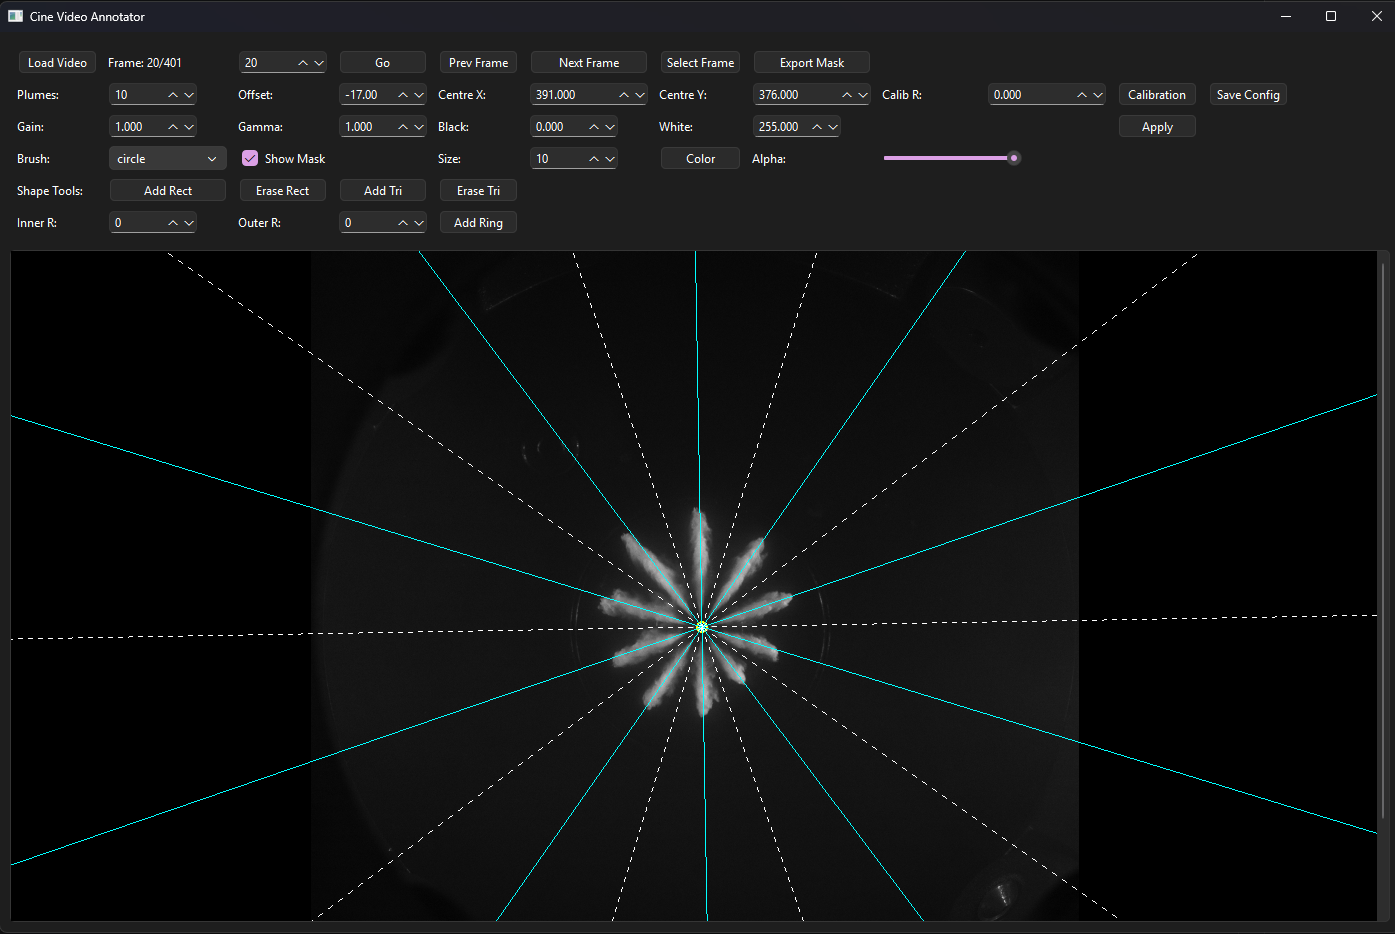
\includegraphics[width=\linewidth]{../images/GUI_gain_1.png}
\end{minipage}
\hfill
\begin{minipage}[t]{0.49\linewidth}
\centering
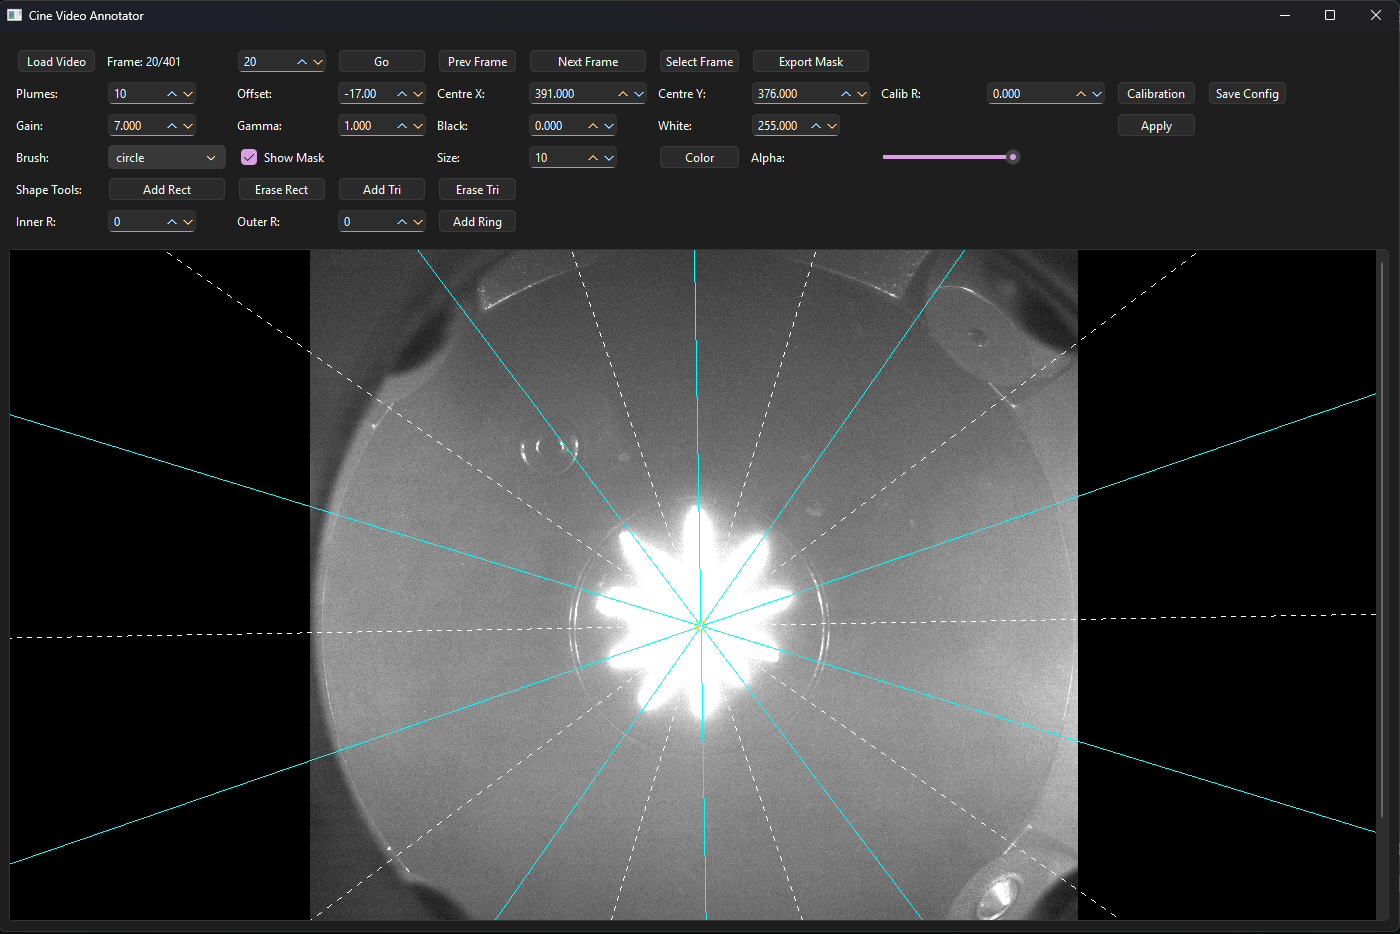
\includegraphics[width=\linewidth]{../images/GUI_gain_7.png}
\end{minipage}
\caption{交互式标定界面中显示的同一喷雾帧，增益分别为 1.0 和 7.0，其余显示参数保持不变。较高增益视图使喷雾周围的明亮光晕更明显，说明显示映射会改变视觉边界感知；这些增益视图仅用于人工检查，不作为定量边界提取输入。}
\label{fig:gui-gain-halo}
\end{figure}

\begin{figure}[t]
\centering
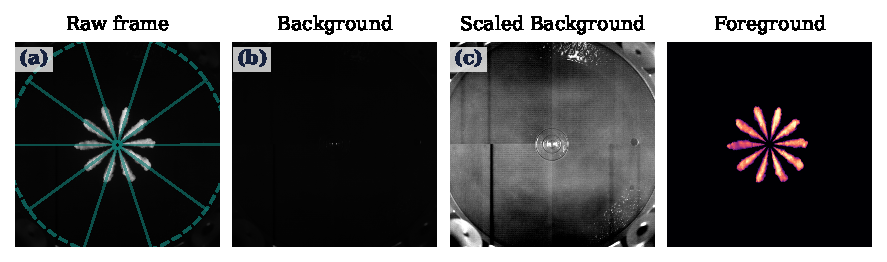
\includegraphics[width=0.92\linewidth]{../images/fig_mie_preproc_background.pdf}
\caption{鲁棒背景阶段的代表帧可视化。（a）原始帧和标定几何；（b）由喷射前帧估计的背景；（c）经对数比背景扣除后的前景表示。}
\label{fig:mie-preproc-background}
\end{figure}

\subsubsection{基于硬件加速的Sobel梯度滤波器进行边缘增强}

第二个贡献是直接作用于整个视频立方体的显式边缘增强高通阶段。
在 \textbf{GPU 加速的 Sobel 滤波器} 中，Sobel 核 \(K_x\) 和 \(K_y\) 只生成一次，并通过 \textbf{二维卷积程序} 应用：
\[
S_t(x,y)=\sqrt{\left(K_x * F_t\right)^2+\left(K_y * F_t\right)^2},
\]
其中，\(K_x\) 和 \(K_y\) 分别是水平和垂直方向的 Sobel 卷积核，\(*\) 表示二维卷积算子，\(F_t\) 是预处理后的前景图像，\(S_t\) 则是得到的梯度幅值。

更细微的效率收益来自 Sobel 核本身的秩-1 结构。
在 \textbf{卷积核构建函数} 中，每个方向核都被显式组装为外积：
\[
K_x = \mathbf{g} \otimes \mathbf{d}_g, \qquad K_y = \mathbf{d}_g \otimes \mathbf{g},
\]
其中 \(\mathbf{g}\) 是离散高斯包络，\(\mathbf{d}_g\) 是它的导数。
外积矩阵的秩恰好为 1，因此二维卷积等价于沿空间轴进行两次一维顺序卷积。
\textbf{秩-1 可分离性测试} 会自动验证这一点，并在条件满足时切换到可分离路径，把 \(k\times k\) 核的每像素乘加开销从 \(O(k^2)\) 降到 \(O(2k)\)。
由于 Sobel 核在构造上就是秩-1，\(K_x\) 和 \(K_y\) 在整个视频立方体上总是以一对一维卷积的形式应用。

随后再次进行稳健缩放，并施加环形几何掩码。
这一步在实现层面很关键，因为它把低对比度灰度喷雾转化为边缘主导的表示，同时让整个操作都停留在 CuPy 后端。
这里的贡献不在于 Sobel 算子本身，而在于把它集成进一条避免反复主机--设备拷贝的批量视频工作流中，为每个羽流准备一致的下游几何处理 \cite{GonzalezWoodsDIP,Szeliski2010Vision}。

\begin{figure}[t]
\centering

\includegraphics[width=0.92\linewidth]{../images/fig_mie_preproc_sobel.pdf}
\caption{边缘增强高通阶段的代表帧可视化。（a）背景扣除后的前景；（b）Sobel 梯度幅值。}
\label{fig:mie-preproc-sobel}
\end{figure}

\begin{figure}[t]
\centering

\includegraphics[width=0.92\linewidth]{../images/fig_threshold_mask_repair_summary.pdf}
\caption{从高通表示到二值喷雾支持的紧凑示例。（a）整个视频环形区域内的高通强度分布，并标出固定支持阈值；（b）代表帧上的单羽流高通条带；（c）固定阈值化得到的原始二值支持；（d）形态学修补后的二值支持，并高亮被添加和移除的像素。}
\label{fig:threshold-mask-repair-summary}
\end{figure}

高通条带不再使用 triangle threshold 进行二值化，因为该规则对接近零的峰值、长尾强度分布以及掩码引入的零值比例都很敏感。
当前实现首先对每个羽流的 \((t,y,x)\) 高通条带体做基于百分位数的最小--最大归一化，把 \(q_{\min}=5\) 和 \(q_{\max}=99.9\) 百分位映射到 0 和 1，并截断范围外的值。
随后在归一化条带上使用单一固定阈值 \(T_{\mathrm{BW}}=0.01\)：
\[
B_p(t,y,x)=\mathbf{1}\!\left[\tilde{H}_p(t,y,x)>T_{\mathrm{BW}}\right].
\]
百分位归一化吸收了不同视频之间的亮度和局部对比度差异，而固定阈值只表示归一化后的边缘响应是否足够强。
图~\ref{fig:threshold-mask-repair-summary}(a) 中标出的阈值，就是归一化强度尺度上的这个固定支持阈值。

当二值支持需要进一步修补时，\textbf{二值羽流视频修补函数}采用先时间体、后单帧的顺序。
对于每个羽流的 \((t,y,x)\) 二值体，流程先用 \(3\times3\times3\) 结构元做 closing，再填孔并保留三维最大连通域；随后对每一帧再保留二维最大连通域。
前一步利用时间邻接性修补短暂断裂，后一步去除每帧中的悬挂碎片。
图~\ref{fig:threshold-mask-repair-summary}(d) 展示了这一修补路径对单帧支持掩码的影响；它应被理解为二值几何度量的稳健化步骤，而不是对原始 Mie 强度场的物理恢复。

\subsubsection{从角度强度信号中确定羽流方向}

预处理完成后，流程不再通过笛卡尔坐标中的轮廓追踪寻找羽流方向。
相反，\textbf{极坐标重参数化程序}会围绕已标定的喷嘴中心做极坐标重参数化。
对于每个像素，
\[
\theta(x,y)=\operatorname{atan2}(y-c_y,\;x-c_x)\bmod 360^\circ,
\]
每帧在角度箱 \(k\) 中的角度信号累积为
\[
A_t(k)=\sum_{(x,y)\in \mathcal{B}_k} I_t(x,y), \qquad
D_t(k)=\frac{A_t(k)}{\#\mathcal{B}_k},
\]
其中 \(\mathcal{B}_k\) 是角度落入箱 \(k\) 的像素集合，\(I_t(x,y)\) 是处理后的前景强度，\(A_t(k)\) 是累积角度信号，\(D_t(k)\) 是平均角度密度，\(\#\mathcal{B}_k\) 则是该箱中的像素数。
在 CuPy 实现中，分箱和加权求和都直接在 GPU 数组上完成，分别由 \textbf{GPU 直方图分箱操作} 和 \textbf{GPU 加权求和操作} 执行。
概念上，这是把 2D 图像径向压缩成一个 1D 角度占用信号；对多孔对齐而言，它比原始帧中的边缘碎片稳定得多 \cite{Szeliski2010Vision}。

\subsubsection{基于傅里叶分析的多孔喷油束自动配准}

随后不是从固定偏移量出发，而是从角度信号的周期性中估计羽流导向角。
设
\[
\bar{A}(k)=\sum_t A_t(k)
\]
为时间求和的角度剖面，设 \(P\) 是已知羽流数目。
\textbf{基于 FFT 的相位对齐函数} 计算 \(\bar{A}\) 的实 FFT，读取羽流谐波 \(P\) 的相位，并将其转换为角度偏移：
\[
\hat{\phi}_0
=
-\frac{\arg\!\left(\mathcal{F}\{\bar{A}\}[P]\right)}{P}\frac{180^\circ}{\pi}.
\]
这正是对齐具有自适应性的原因：代码使用当前数据集中观测到的谐波相位，而不是为每条记录手动假定一个参考角。
\textbf{多孔几何构建脚本} 随后构造羽流方向
\[
\phi_p=\frac{360^\circ p}{P}-\hat{\phi}_0, \qquad p=0,\dots,P-1,
\]
并结合三角阈值占用掩码和短间隙填充来排除空角扇区。
FFT 本身是标准方法；这里的贡献在于利用已知喷油器多孔数，把角度密度信号转成一条自动羽流配准规则 \cite{CooleyTukey1965FFT,Szeliski2010Vision}。

同一个 occupied-angle mask 还可以给出一个简单的锥角代理量。
做法是把 bin-wise 掩码视为定义在 \([0,360^\circ)\) 上的周期信号，把跨越 \(0^\circ/360^\circ\) 边界的 \texttt{True} 段合并，再把每个连续段长度从 bins 转成角度。
得到的角宽量化了每条羽流在整段记录中所占据的角度支持范围。
我们同时报告总占用角和连续段平均宽度；后者可以作为一个粗略的锥角代理，因为它无需逐帧单独拟合边缘，就能概括羽流的平均角向展开宽度。

\begin{figure}[t]
\centering

\includegraphics[width=0.92\linewidth]{../images/fig_angular_occupancy.pdf}
\caption{极坐标角度占用分析。（a）逐帧角度信号热图；（b）时间求和角度剖面，浅色竖线标记估计的羽流导向角；（c）通过角度剖面阈值化和短间隙填充得到的占用角度掩码；（d）FFT 谐波谱，喷孔数以虚线竖线标出，并标注计算得到的角度偏移。}
\label{fig:angular-occupancy}
\end{figure}

\begin{figure}[t]
\centering

\includegraphics[width=0.92\linewidth]{../images/fig_angular_mask_comparison.png}
\caption{基于 FFT 的羽流配准所得占用角度掩码，以两种坐标系呈现。（a）笛卡尔视图：喷雾在整段视频中占用的角度区间以白色扇形渲染，叠加喷嘴中心（红叉）和视野边界（红色虚圆）；标注信息包括总占用角度、检测到的区段数及锥角代理值。（b）极坐标展开视图：每列对应一个 0.5$^\circ$ 角度区间，白色表示有喷雾，绿色水平线标记视野半径；各区段宽度（逐羽流锥角估计）标注于顶部。}
\label{fig:angular-mask-comparison}
\end{figure}

\subsubsection{逆仿射映射和羽流条带提取}

一旦得到目标角度，每条羽流都会被重映射到一个共同的喷嘴左侧条带坐标系中。
每个羽流角 \(\phi_p\) 定义了一个旋转加平移变换，把喷嘴放到输出条带的左边缘和中间高度；重映射通过 \textbf{逆仿射映射生成器} 中实现的逆关系完成：
\[
\begin{bmatrix}
x_{\mathrm{src}}\\y_{\mathrm{src}}
\end{bmatrix}
=
\mathbf{A}^{-1}
\!\left(
\begin{bmatrix}
u\\v
\end{bmatrix}
-\mathbf{b}
\right),
\qquad
\mathbf{A}
=
\begin{bmatrix}
\cos\phi_p & \sin\phi_p\\
-\sin\phi_p & \cos\phi_p
\end{bmatrix},
\qquad
\mathbf{b}=\mathbf{t}-\mathbf{A}\mathbf{c},
\]
其中 \(\mathbf{c}=(c_x,c_y)^\top\) 是喷嘴中心，\(\mathbf{t}\) 是条带原点平移。
对每条羽流，\textbf{X/Y 坐标逆空间图} 只需预先计算一次，方法是先用 \textbf{正向仿射变换构建器} 生成，随后由 \textbf{GPU 视频重采样程序} 用最近邻、双线性、双三次或 Lanczos 核对整个视频立方体采样。
这些图保存的是源图像采样坐标，而不是喷雾强度：X 图像素值给出输出条带像素在源图像中采样的 \(x\) 坐标，Y 图则保存对应的 \(y\) 坐标。
多孔流程在重映射后应用固定条带尺寸 \textbf{标准化条带尺寸} 和三角形羽流掩码。
每个羽流角只需预计算一次逆映射，因此逐帧开销与旋转无关；后续所有度量都在同一个局部条带坐标系里测量 \cite{Szeliski2010Vision}。

\begin{figure}[t]
\centering

\includegraphics[width=0.92\linewidth]{../images/fig_efficient_rotation.pdf}
\caption{逆仿射重映射和条带坐标中的几何度量。（a）旋转后的单羽流高通条带，局部孔口位置、内半径、$S_{\mathrm{CDF}}$（CDF 穿深前沿 $\hat{x}_p$，定义见第~3.4.8~节）、$S_{\mathrm{BW,x}}$（轴向二值穿深）和 $R_{\mathrm{BW}}$（极坐标二值穿深 $R_p$，定义见第~3.4.9~节）叠加在同一坐标系中；（b）重映射后施加的三角喷雾掩码；（c）逆映射数组的紧凑预览，其中颜色通道编码了每个输出条带像素的源图像采样坐标。}
\label{fig:efficient-rotation}
\end{figure}

\subsubsection{来自对齐羽流条带的鲁棒 CDF 穿深}

穿深估计器刻意基于累积强度支持，而不是单个最亮像素或最外层的孤立团块。
对于每个羽流条带 \(I_p(t,y,x)\)，\textbf{逐羽流 CDF 穿深估计器}先沿横向坍缩，
\[
H_p(t,x)=\sum_y I_p(t,y,x),
\]
再对每一帧减去左边缘基线、截断负值，并通过自动阈值、最大连通域清理和二值开运算生成支持掩码。
在该支持区域内，\textbf{轴向 CDF 前沿定位器}构造轴向累积分布
\[
C_p(t,x)=\frac{\sum_{\xi \le x} \tilde{H}_p(t,\xi)}{\sum_{\xi} \tilde{H}_p(t,\xi)+\varepsilon},
\]
其中 \(\tilde{H}_p(t,\xi)\) 是扣除基线并清理后的横向强度和，\(\varepsilon\) 用于防止除零，而 \(C_p(t,x)\) 是得到的轴向累积分布。
随后，穿深前沿 \(\hat{x}_p(t)\) 被定义为满足
\[
\hat{x}_p(t)=\min \{x : C_p(t,x)\ge q\},
\]
的最小位置，其中分位数阈值在本文整个批量归档中固定为 \(q=0.995\)，即 \codepath{mie\_multi\_hole.py} 中的 \texttt{upper\_quantile\_cdf = 1 - 5e-3}。
可复用库函数在交互式测试时保留一个更低的默认值；本文所有定量结果都使用批处理脚本写入归档的 \(q=0.995\)。由于按列求和的强度 CDF 在前沿处急剧上升，恢复出的前沿在该取值的邻域内对 \(q\) 不敏感；\(q=0.995\) 被选作一个保守的前沿定义，用以排除液核之外微弱的散射光晕，而非作为调过的超参数。
随后减去内半径，把距离表达成相对于喷嘴环面的量，并进行显式轨迹清理。
这一步清理不是通过 cumulative maximum 把所有回退值抬高，而是在检测到第一个非物理后退跳跃后直接截断尾部：
\[
\Delta \hat{x}_p(j)=\hat{x}_p(j+1)-\hat{x}_p(j),\qquad
j_p^\star=\min\{j:\Delta \hat{x}_p(j)<0\},
\]
\[
\hat{x}_p(t)\leftarrow \mathrm{NaN}\quad \text{for}\quad t\ge j_p^\star .
\]
在实现中，截断从第一个负差分附近的帧开始，因此可能牺牲后面较弱的重新出现信号；这是一个保守选择，用来避免把孤立噪声尖峰或边界反射误认为真实的穿深回撤。
尾部截断之后，脚本构建有效帧掩码，并用 \texttt{remove\_short\_true\_runs(..., min\_len=5)} 去掉孤立的短区段。
这个 CDF 前沿是工作流在实践中的主要贡献之一：它对断裂的前缘像素远不如朴素的最大索引定义敏感，同时仍然给出与标准柴油喷雾用法一致的穿深量 \cite{Dent1971Penetration,HiroyasuArai1990,NaberSiebers1996}。

\begin{figure}[t]
\centering
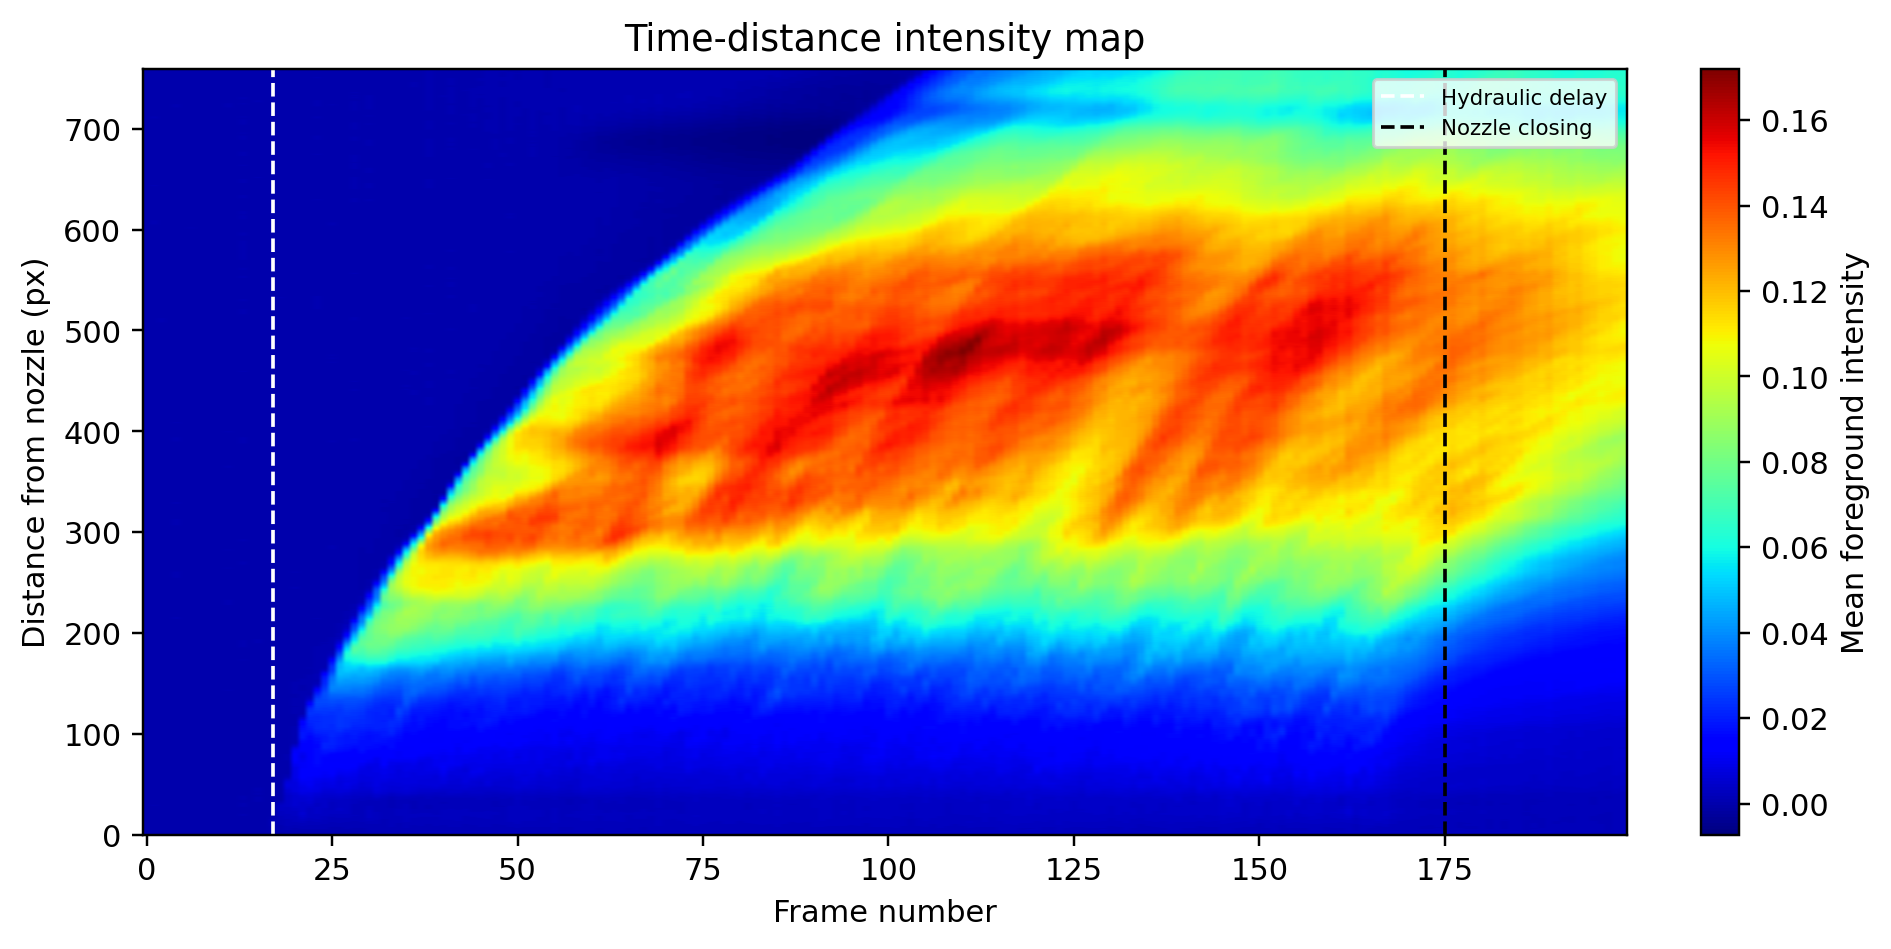
\includegraphics[width=0.92\linewidth]{../images/td_map.png}
\vspace{2pt}
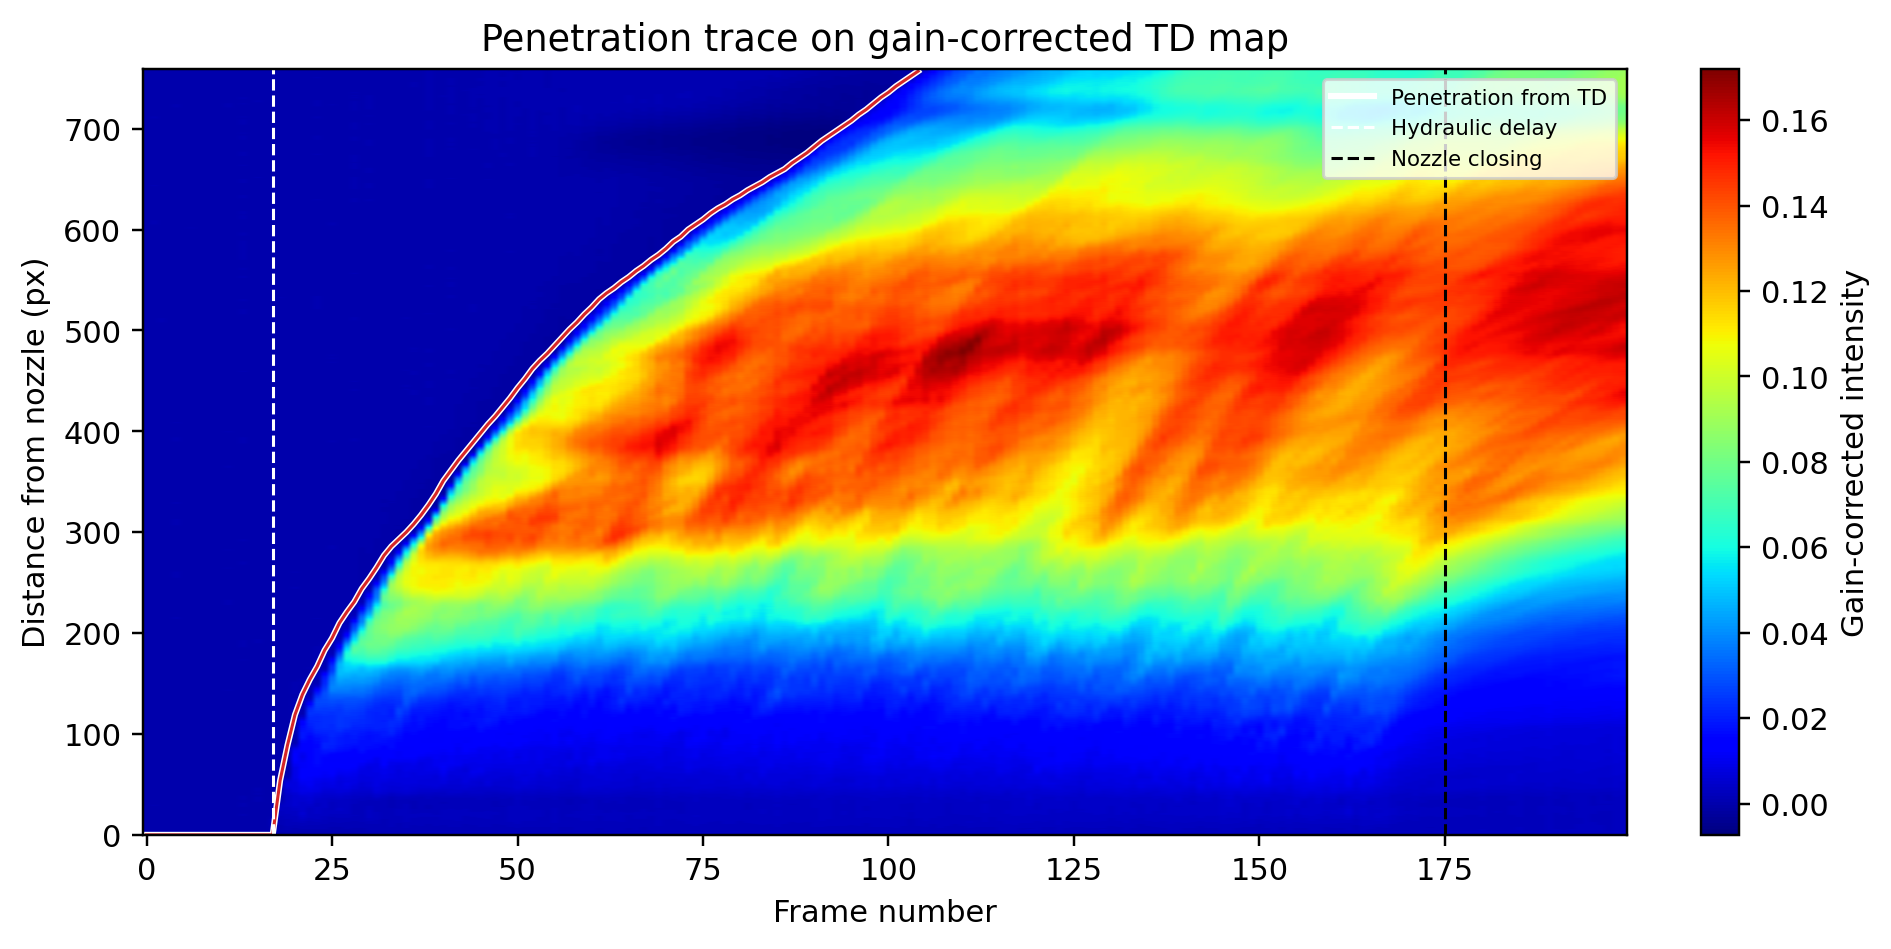
\includegraphics[width=0.92\linewidth]{../images/penetration_td.png}
\caption{代表性单羽流的时间--距离（TD）强度图，展示 CDF 穿深提取过程（单孔录像，仅用于说明；相同处理流程适用于全部喷嘴族）。上图：TD 图将羽流条带沿横向折叠，以二维形式呈现轴向喷雾随时间的发展；液压延迟（白色虚线）和喷嘴关闭（黑色虚线）已标注。下图：在增益校正 TD 图上叠加 CDF 穿深前沿 $\hat{x}_p(t)$（粉色曲线），分位数阈值 $q=0.995$。}
\label{fig:td-map-penetration}
\end{figure}

\subsubsection{边界度量和几何代理}

二值化后的羽流条带也会传给 \textbf{次级特征提取器}，后者计算若干次要观测量。
投影面积为
\[
A_p(t)=\sum_{x,y} B_p(t,y,x).
\]
轴向二值穿深通过占用像素数超过阈值的最右列得到，而极坐标穿深则从上边界点云和下边界点云定义为
\[
R_p(t)=\max\!\left(
\max_i \sqrt{x_{u,i}^2+y_{u,i}^2},
\max_j \sqrt{x_{l,j}^2+y_{l,j}^2}
\right).
\]
代码还会存储一个类体积的几何代理：
\[
V_p(t)=x_{\mathrm{scale}} \frac{\pi}{4}\sum_x \left(w_u(t,x)+w_l(t,x)\right)^2,
\]
其中 \(w_u\) 和 \(w_l\) 分别是上半宽和下半宽，而 \(x_{\mathrm{scale}}=1/\cos((180^\circ-\theta_{\mathrm{umb}})/2)\) 在需要时补偿伞角倾斜。
这个量不是三维重建，而是把二值投影截面解释成一个轴对称包络后得到的几何代理。
脚本还会导出上下界版本，
\[
V_{p,\max}(t)=\pi x_{\mathrm{scale}}\sum_x \max(w_u,w_l)^2,\qquad
V_{p,\min}(t)=\pi x_{\mathrm{scale}}\sum_x \min(w_u,w_l)^2,
\]
它们分别用两个半宽中的较大值和较小值作为局部有效半径，用于记录上下边界不对称时该代理的可能范围。
锥角代理通过两种方式计算：一是对局部边界角度取平均
\[
\alpha_{\mathrm{avg}}(t)=\overline{\arctan(y_u/x_u)}-\overline{\arctan(y_l/x_l)},
\]
二是拟合固定截距的边界线并计算
\[
\alpha_{\mathrm{lg}}(t)=\arctan(m_u)-\arctan(m_l).
\]
最后，靠近喷嘴的开启和关闭时刻由喷油器附近的一个小检测窗口推断得到。
检测逻辑对该窗口内的平均块强度进行鲁棒归一化，随后应用双阈值滞后方案（高阈值 0.50，低阈值 0.10），并标记检测到的有效喷射区间；图~\ref{fig:nozzle-timing} 展示了一条典型的时序信号及其液压延迟与喷嘴关闭事件。

\begin{figure}[t]
\centering
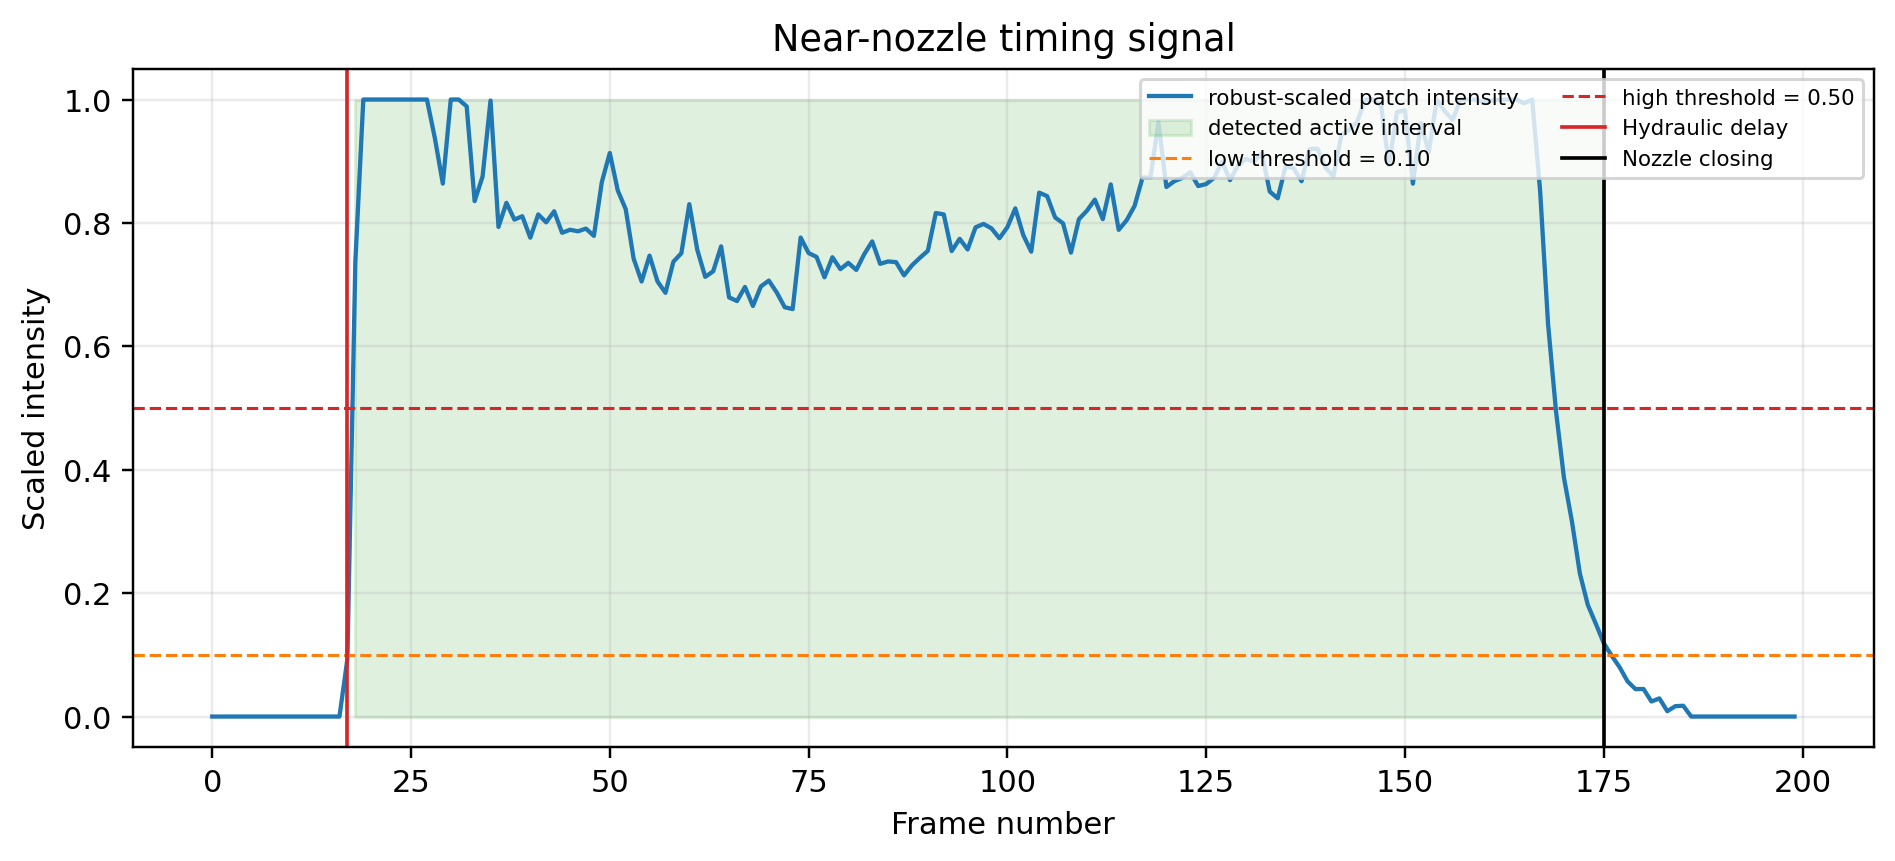
\includegraphics[width=0.92\linewidth]{../images/nozzle_timing.png}
\caption{用于检测液压延迟和喷嘴关闭事件的近喷嘴时序信号。鲁棒归一化后的块强度（蓝色）在液压延迟处（红色竖实线）升过高阈值（红色虚线），在喷嘴关闭处（黑色竖实线）降至低阈值（橙色虚线）以下；检测到的有效喷射区间以绿色高亮显示。单孔录像，仅用于说明；相同检测算法适用于全部喷嘴族。}
\label{fig:nozzle-timing}
\end{figure}

这些度量之所以重要，是因为它们把每条对齐后的条带压缩成一个紧凑的几何状态向量；不过，本文的下游建模仍然以穿深为中心，因为在现有分析里它是支持最充分的目标 \cite{Linne2013SprayImaging,LefebvreMcDonell2017}。

\subsection{无像素级真值的边界提取}

本文的喷雾边界提取依赖梯度增强、形态学清洗和物理一致性校验。Mie 散射图像中，液滴散射产生强局部对比度，使喷雾与背景分界清晰，上述方案与这一成像特性相符。

本文未进行逐像素边界标注。对高速 Mie 时间序列进行此类标注需要大量人工工作，且所得标签反映的是标注者的主观判断，而非客观物理真值。喷雾边界随雾化和液滴破碎持续变化，不存在唯一的像素级真值。因此，需要参考掩码的 IoU 和 F1 等指标在此不适用。

本文通过叠加覆盖检查、时间连续性验证以及多个几何代理量之间的一致性来评估边界提取的可靠性。这一评估方式与本文目标相符：稳定提取贯穿距离、锥角和边界包络等可观测量，而非训练语义分割模型。相关定量证据在第~5~章呈现。

\begin{figure}[t]
\centering
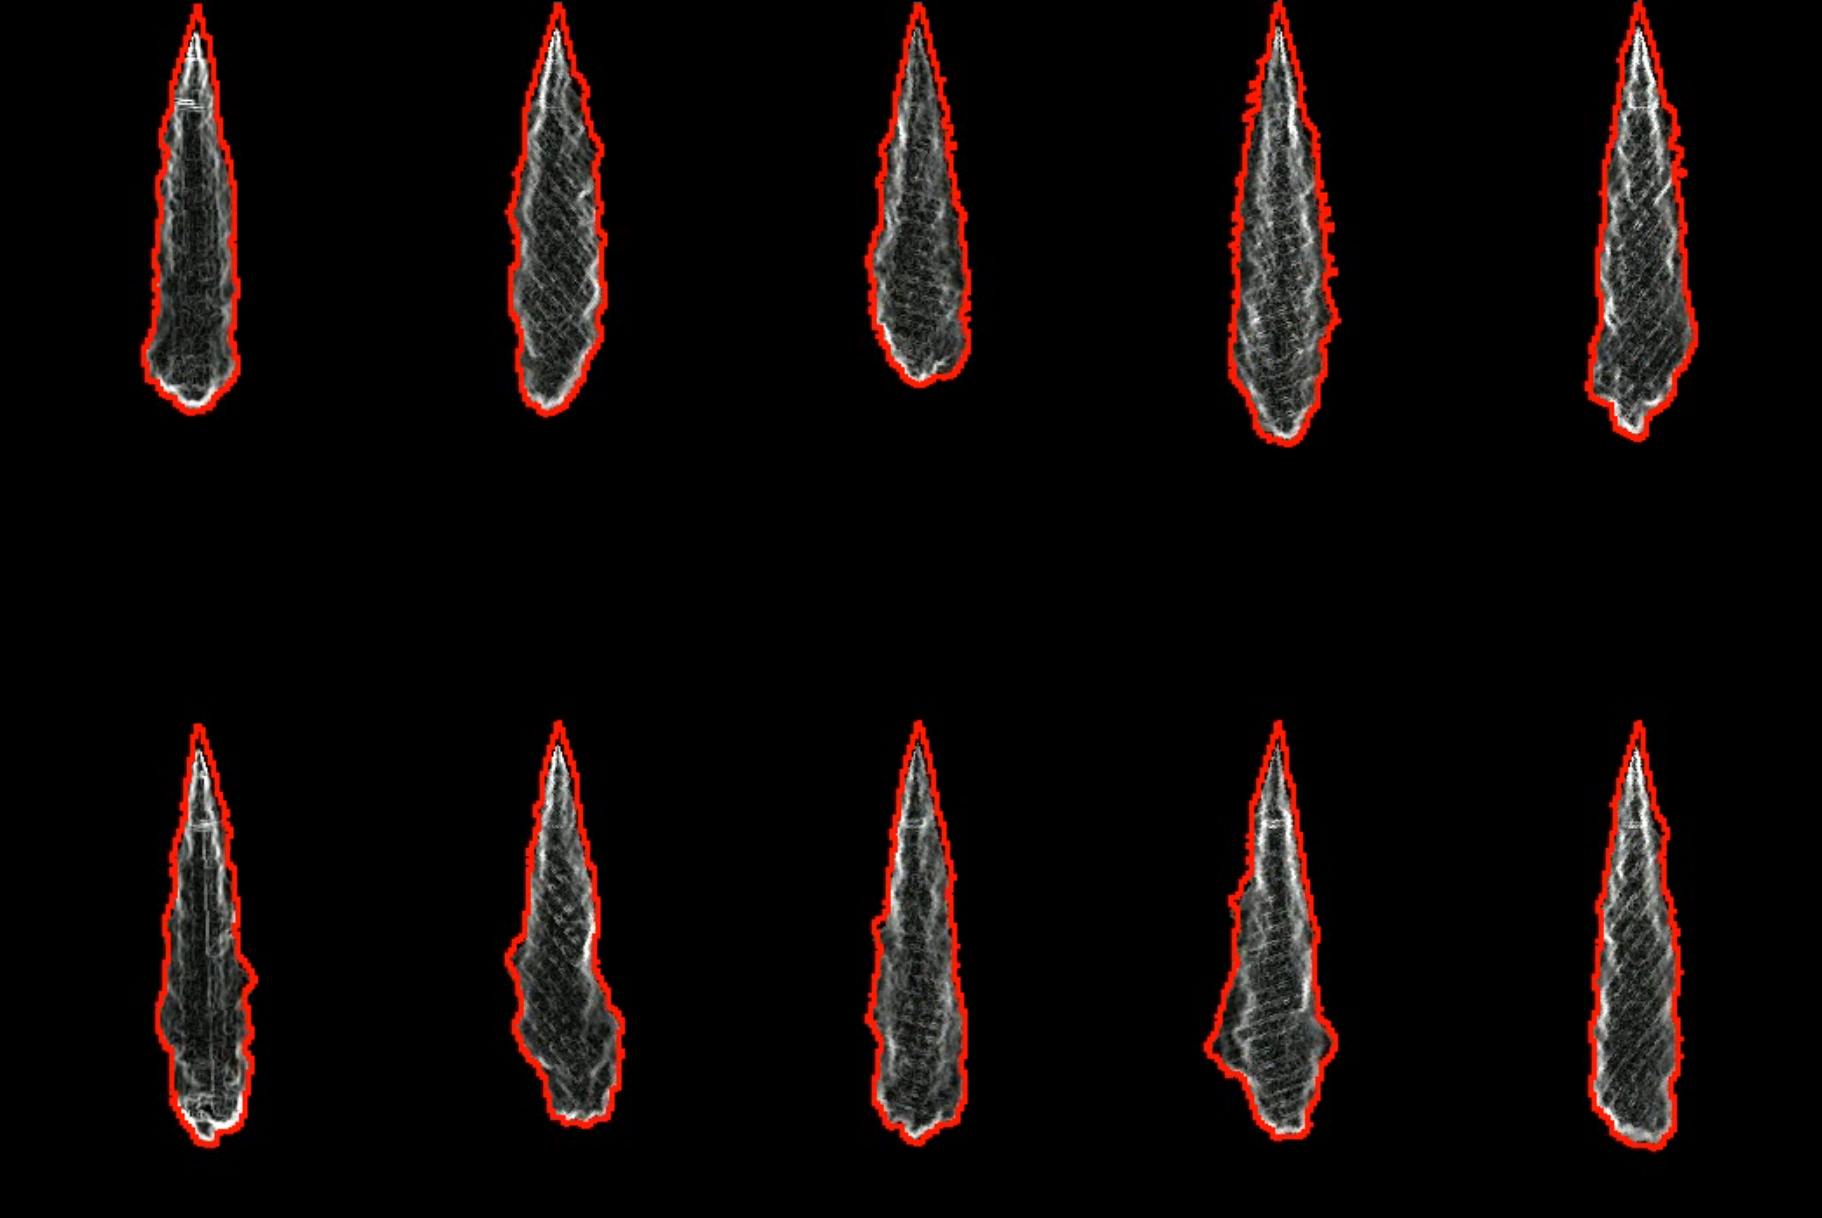
\includegraphics[width=0.92\linewidth]{../images/fig_mie_segmentation_boundary_overlay.png}
\caption{喷雾边界提取结果的可视化检查。灰度前景由原始 Mie 图像经对数背景除法、Sobel 梯度增强和最近邻旋转重映射得到；红色轮廓是从二值支持图像导出的 BW 边界。该叠加图表明，边界代理主要跟随局部对比度变化形成的有效液相包络，而不是依赖单个最前端亮点。}
\label{fig:mie-segmentation-boundary-overlay}
\end{figure}

\begin{figure}[t]
\centering

\includegraphics[width=0.92\linewidth]{../images/fig_mie_metrics_summary.pdf}
\caption{对齐和二值化后的主要定量输出示例。（a）三种穿深描述符随帧索引变化；（b）两种锥角代理量；（c）代表性羽流的二值条带最大投影，并标出靠近喷嘴的开启和关闭帧。}
\label{fig:mie-metrics-summary}
\end{figure}
